We split this section into four parts: \textbf{Data, Preprocessing, Data Augmentation} and \textbf{Model}.
\subsection{Data}
We used \textbf{ESC-50} dataset\cite{ESC50} that is most commonly used in environmental sounds classification. The dataset consists of 5-second-long audio segment which can be classified into one of 50 sound events, e.g., dog barks, sea waves sound, rain sound.
The 50 sound event class could loosely arranged into 5 major categories(fig.\ref{esc}): \textbf{Animals, Natural Soundscapes \& Water Sound, Human(Non-Speech Sounds), }and \textbf{Exterior/Urban Noises}. Each categories include 10 class.
The dataset included 2000 environmental audio sample(with 40 example per class).
\begin{figure}[H]
\centering
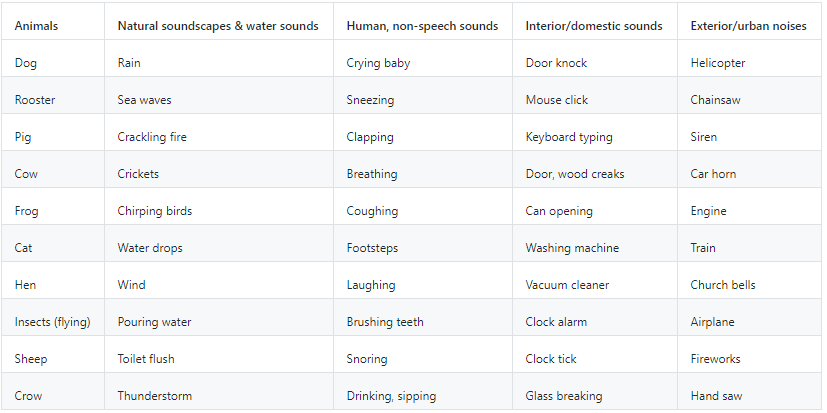
\includegraphics[width=\textwidth]{./graph/ESC50-categories.PNG} 
\caption{ESC50 - Categories}
\label{esc}
\end{figure}
\subsection{Preprocessing}\label{pre}
The data we got is in the form of wave file, so that we can not feed it into CNN directly. We converted environment sound waveform to spectrogram and MFCC. 
These two can seem as visual representation of audio. We often use heatmap to visualize spectrogram and MFCC. X-axis is time, Y-axis is frequency of audio and color shows frequency strength of audio at that moment. 
Most difference of spectrogram and MFCC is that the latter scaled based on human hearing where the former only do log scaled.
Fig.\ref{wave} and fig.\ref{sp} show the clear difference between waveform and spectrogram.
\begin{figure}[H]
\begin{minipage}[t]{0.5\textwidth}
\centering
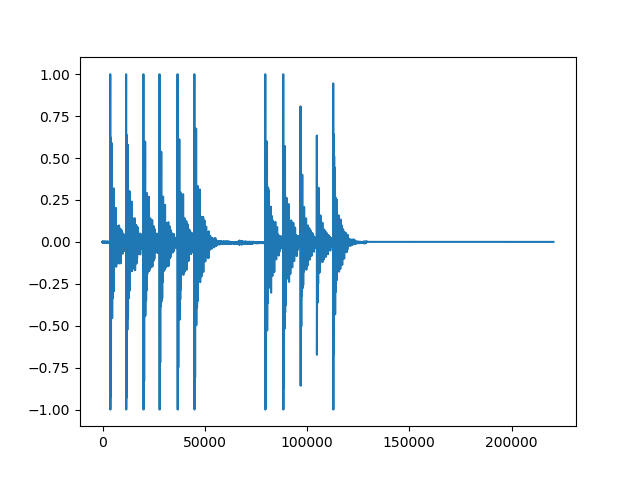
\includegraphics[width=\textwidth]{./graph/door_wood_knock_original_wave.png} 
\caption{Door Knock Waveform}
\label{wave}
\end{minipage}
\begin{minipage}[t]{0.5\textwidth}
\centering
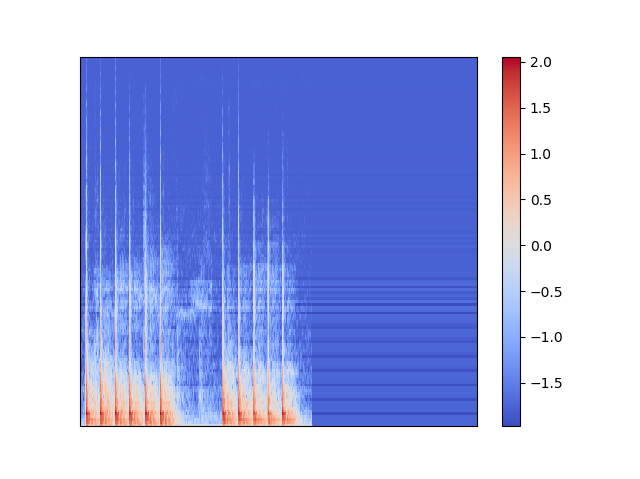
\includegraphics[width=\textwidth]{./graph/door_wood_knock_original_melsp.png} 
\caption{Door Knock Mel-Spectrogram}
\label{sp}
\end{minipage}
\end{figure}

\subsection{Data Augmentation}
Due to the lack of training sample, we also perform three easy transformation to extend our dataset. 
First is \textbf{white noise}(fig.\ref{WHwave}\&\ref{WHsp}), we add white noise which is a random signal having equal intensity at different frequency as the background.
That make sense because that also lots of noise in real world. Second thing we did is \textbf{sound shift}(fig.\ref{SSTwave}\&\ref{SSTsp}). Smoothly shift signal in random rate. For example, if dog barks at time = 1s, we will shift this event to time = 3s with same amplitude, length\ldots. 
The last augmentation we did is \textbf{stretching sound}(fig.\ref{SSwave}\&\ref{SSsp}), which modify signal sound length to make sound play a little faster.
\begin{figure}[H]
\begin{minipage}[t]{0.5\textwidth}
\centering
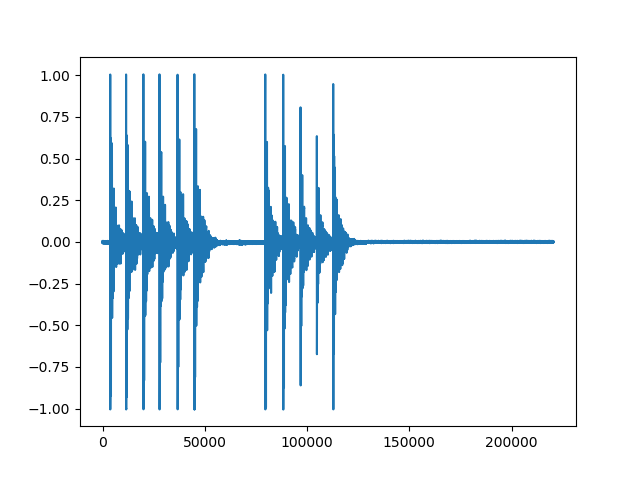
\includegraphics[width=\textwidth]{./graph/door_wood_knock_WhiteNoise_wave.png} 
\caption{Door Knock Waveform(White Noise)}
\label{WHwave}
\end{minipage}
\begin{minipage}[t]{0.5\textwidth}
\centering
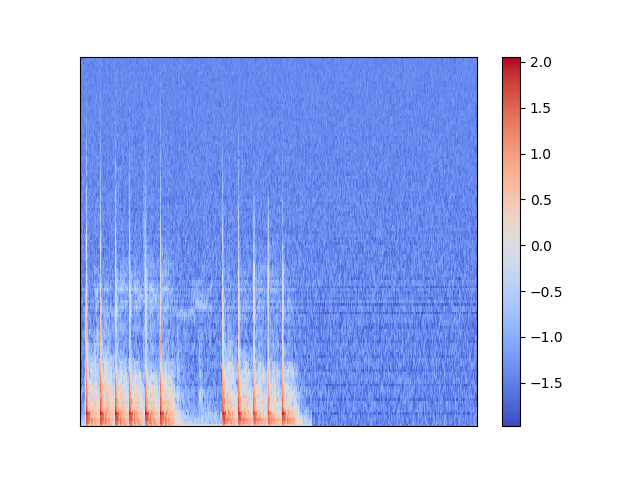
\includegraphics[width=\textwidth]{./graph/door_wood_knock_WhiteNoise_melsp.png} 
\caption{Door Knock Mel-Spectrogram(White Noise)}
\label{WHsp}
\end{minipage}
\end{figure}

\begin{figure}[H]
\begin{minipage}[t]{0.5\textwidth}
\centering
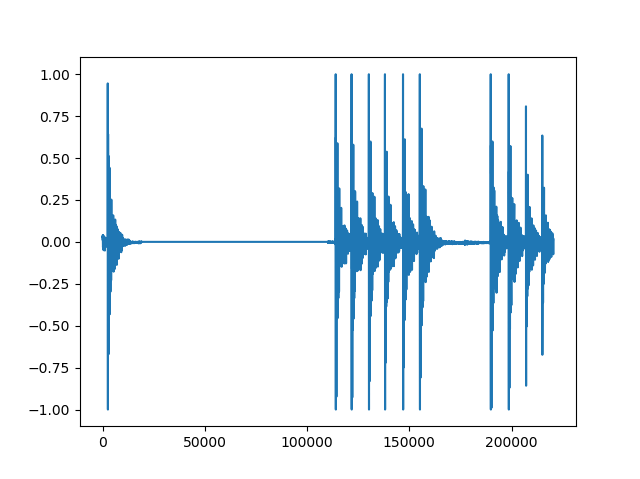
\includegraphics[width=\textwidth]{./graph/door_wood_knock_SoundShift_wave.png} 
\caption{Door Knock Waveform(Sound Shift)}
\label{SSTwave}
\end{minipage}
\begin{minipage}[t]{0.5\textwidth}
\centering
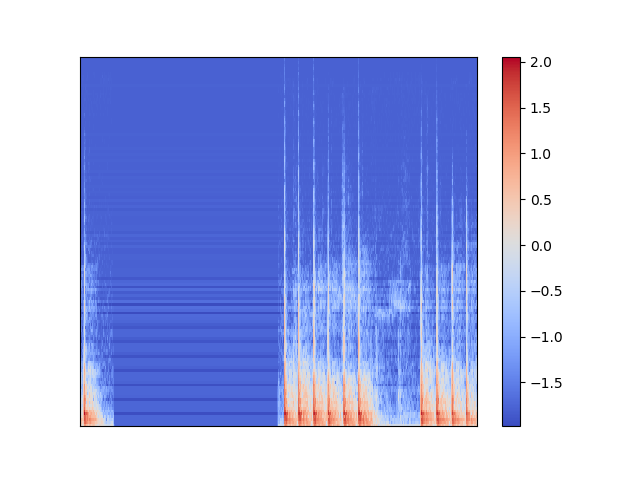
\includegraphics[width=\textwidth]{./graph/door_wood_knock_SoundShift_melsp.png} 
\caption{Door Knock Mel-Spectrogram(Sound Shift)}
\label{SSTsp}
\end{minipage}
\end{figure}

\begin{figure}[H]
\begin{minipage}[t]{0.5\textwidth}
\centering
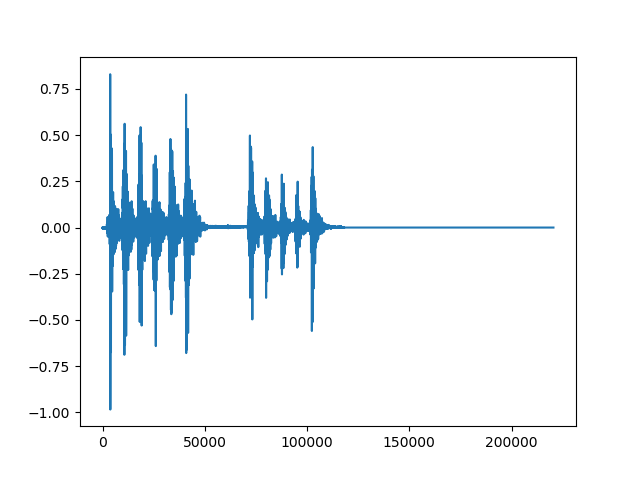
\includegraphics[width=\textwidth]{./graph/door_wood_knock_StretchSound_wave.png} 
\caption{Door Knock Waveform(Stretch Sound)}
\label{SSwave}
\end{minipage}
\begin{minipage}[t]{0.5\textwidth}
\centering
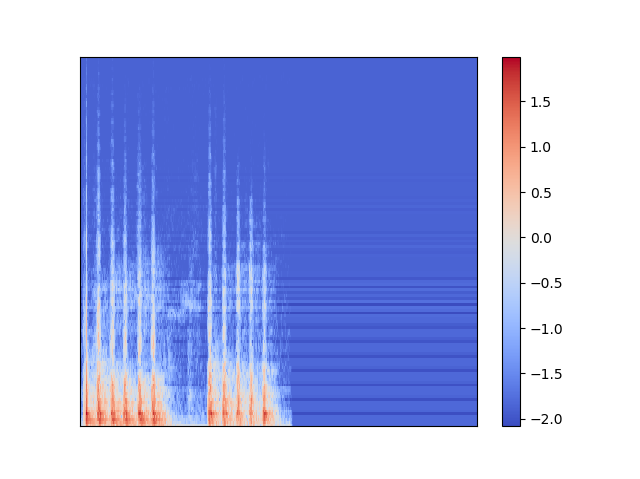
\includegraphics[width=\textwidth]{./graph/door_wood_knock_StretchSound_melsp.png} 
\caption{Door Knock Mel-Spectrogram(Stretch Sound)}
\label{SSsp}
\end{minipage}
\end{figure}
\subsection{Model}
We use convolutional Neural Network(CNN) as our model. Filter is a important component in CNN, which can extract 
significant part in an image. We adopt many filters with different size and amount, and expect to produce greater 
performance for environment sound classification. Against the number of filters, we tried 32,64 and 128. For the size of filter,
(1,8)、(8,1)、(1,16)、(16,1)、(1,32)、(32,1)、(1,64)、(64,1) have been used because in environment sound classification, most important features
are time and frequences, and it contruct an feature map like image. 
However, sinece we bulid CNN with many layers, we use zero padding to avoid descreasing output in each layer. Finally, we can see form the graph,
which show the model is more precisely when epochs increase and get better performance. Due to cost of time, epoch is only set max to 100.
We also tried CNN with less layer, but the performance drop a lot. Showing that deep neural network is necessary. 
